% !TEX program=lualatex
\RequirePackage{luatex85}
\documentclass[10pt,tikz]{standalone}

\usepackage{luatextra} % also loads fixltx2e, fontspec, xunicode
\usepackage{microtype} % Slightly tweak font spacing for aesthetics
\usepackage{mathtools}
\usepackage{amsmath}
\usepackage{unicode-math}
\usepackage{xcolor}

\usepackage{tikz}
\usetikzlibrary{shapes,arrows,positioning,calc,decorations.pathmorphing}

\setmainfont{TeX Gyre Heros}
\setmathfont{Latin Modern Math}

\definecolor{colorR}{RGB}{228,26,28}    % RED
\definecolor{colorB}{RGB}{55,126,184}   % BLUE
\definecolor{colorG}{RGB}{77,175,74}    % GREEN
\definecolor{colorP}{RGB}{152,78,163}   % PURPLE
\definecolor{colorO}{RGB}{255,127,0}    % ORANGE
\definecolor{colorY}{RGB}{255,255,51}   % YELLOW
\definecolor{colorBn}{RGB}{166,86,40}   % BROWN
\definecolor{colorPk}{RGB}{247,129,191} % PINK
\definecolor{colorGy}{RGB}{153,153,153} % GRAY
\definecolor{maroon}{RGB}{140,29,64}

\tikzstyle{line}=[draw, -stealth', line width=0.8pt]
\tikzstyle{lab}=[font=\footnotesize,pos=0.5,inner sep=0.1pt,sloped,above=1.5mm]
\tikzstyle{ref}=[sep=0.1]

\begin{document}
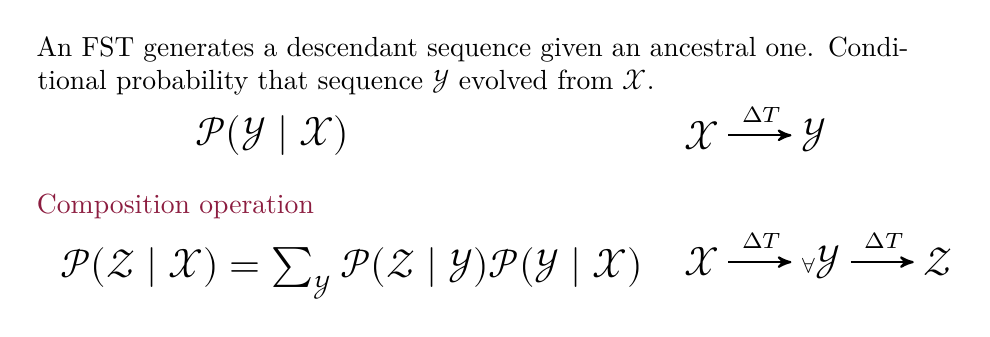
\begin{tikzpicture}[node distance=8mm, auto]

\node (leg1)[text width=11cm] {An FST generates a descendant sequence given an ancestral one. Conditional probability that sequence $\mathcal{Y}$ evolved from $\mathcal{X}$.};

\node[below right=5mm and 20mm of leg1.west] (P1) {\Large $\mathcal{P(Y \mid X)}$};

\node[right=40mm of P1] (x) {\Large $\mathcal{X}$};
\node[right=of x] (y) {\Large $\mathcal{Y}$};
\path[line] (x) to node[lab] {$\mathcal{\Delta }T$} (y.west);

%\node[right=18mm of y] (eg1) {GGC};
%\node[right=of eg1] (eg2) {GTC};
%\path[line] (eg1) to node[lab] {ΔT} (eg2.west);

%%%%%%%%%%%%%%%%%%%%%%%%%%%%%%%%%%%%%%%%%%%%%%%%%%%%%%%%%%%%%%%%%%%%%%%%%%%%%%%%%%%

\node[below right=15mm and -0.1mm of leg1.west] (leg2) {\textcolor{maroon}{Composition operation}};

\node[below right=4mm and 3mm of leg2.west] (P2) {\Large $\mathcal{P(Z \mid X) = \sum_{Y} P(Z \mid Y)P(Y \mid X)}$};

\node[below=10mm of x] (x1) {\Large $\mathcal{X}$};
\node[right=of x1] (y1) {{\footnotesize $\forall$}\Large $\mathcal{Y}$};
\node[right=of y1] (z1) {\Large $\mathcal{Z}$};
\path[line] (x1) to node[lab] {$\mathcal{\Delta }T$} (y1.west);
\path[line] (y1) to node[lab] {$\mathcal{\Delta }T$} (z1.west);

%\node[below=3mm of eg1] (eg3) {GGC};
%\node[below=3mm of eg2] (eg4) {GTC};
%\node[right=of eg4] (eg5) {GTG};
%\path[line] (eg3) to node[lab] {ΔT} (eg4.west);
%\path[line] (eg4) to node[lab] {ΔT} (eg5.west);

%\node[above=0.1mm of x] {};

\end{tikzpicture}
\end{document}